\documentclass[journal,12pt,onecolumn]{IEEEtran}
\usepackage{cite}
\usepackage{graphicx}
\usepackage{amsmath,amssymb,amsfonts,amsthm}
\usepackage{algorithmic}
\usepackage{graphicx}
\usepackage{textcomp}
\usepackage{xcolor}
\usepackage{txfonts}
\usepackage{listings}
\usepackage{enumitem}
\usepackage{mathtools}
\usepackage{gensymb}
\usepackage{comment}
\usepackage[breaklinks=true]{hyperref}
\usepackage{tkz-euclide} 
\usepackage{listings}
\usepackage{gvv}                                        
%\def\inputGnumericTable{}                                 
\usepackage[utf8]{inputenc} 
\usetikzlibrary{arrows.meta, positioning}
\usepackage{xparse}
\usepackage{color}                                            
\usepackage{array}                                            
\usepackage{longtable}                                       
\usepackage{calc}                                             
\usepackage{multirow}
\usepackage{multicol}
\usepackage{hhline}                                           
\usepackage{ifthen}                                           
\usepackage{lscape}
\usepackage{tabularx}
\usepackage{array}
\usepackage{float}
\newtheorem{theorem}{Theorem}[section]
\newtheorem{problem}{Problem}
\newtheorem{proposition}{Proposition}[section]
\newtheorem{lemma}{Lemma}[section]
\newtheorem{corollary}[theorem]{Corollary}
\newtheorem{example}{Example}[section]
\newtheorem{definition}[problem]{Definition}
\newcommand{\BEQA}{\begin{eqnarray}}
\newcommand{\EEQA}{\end{eqnarray}}
\usepackage{float}
%\newcommand{\define}{\stackrel{\triangle}{=}}
\theoremstyle{remark}
\usepackage{circuitikz}
\usepackage{tikz}
\title{GATE MA 2021}
\author{EE25BTECH11030-AVANEESH}
\begin{document}

\maketitle

% General Aptitude (GA) Section
\section*{General Aptitude (GA)}
\subsection*{Q.1 -- 5 Multiple Choice Questions (MCQ), carry ONE mark each (for each wrong answer: $-1/3$).}
\begin{enumerate}
%1
    \item The ratio of boys to girls in a class is 7 to 3. Among the options below, an acceptable value for the total number of students in the class is:
    \begin{enumerate}
        \item 21
        \item 37
        \item 50
        \item 73
    \end{enumerate}
    \hfill(GATE MA 2021)
%2
    \item A polygon is convex if, for every pair of points, P and Q belonging to the polygon, the line segment PQ lies completely inside or on the polygon. Which one of the following is NOT a convex polygon?
    \begin{enumerate}
        \begin{figure}[H]
            \item  
\includegraphics[width=0.2\columnwidth]{figs/opt1.png}
            \item 
\includegraphics[width=0.2\columnwidth]{figs/opt2.png}
            \item 
\includegraphics[width=0.2\columnwidth]{figs/opt3.png}
            \item 
\includegraphics[width=0.2\columnwidth]{figs/opt4.png}
    \caption*{Q.no 9 options}
    \label{fig:q9options}
    \end{figure}
        
    \end{enumerate}
\hfill(GATE MA 2021)
%3
    \item Consider the following sentences:
    (i) Everybody in the class is prepared for the exam.\\
    (ii) Babu invited Danish to his home because he enjoys playing chess.\\
    Which of the following is the CORRECT observation about the above two sentences?
    \begin{enumerate}
        \item (i) is grammatically correct and (ii) is unambiguous
        \item (i) is grammatically incorrect and (ii) is unambiguous
        \item (i) is grammatically correct and (ii) is ambiguous
        \item (i) is grammatically incorrect and (ii) is ambiguous
    \end{enumerate}
\hfill(GATE MA 2021)
%4
    \item A circular sheet of paper is folded along the lines in the directions shown. The paper, after being punched in the final folded state as shown and unfolded in the reverse order of folding, will look like \_\_\_\_\_\_\_\_.
    \begin{figure}[H]
        \centering
        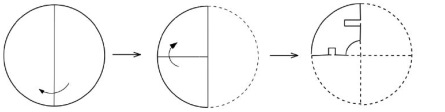
\includegraphics[width=0.5\linewidth]{figs/Q4.png}
        \caption{Q.4.}
        \label{fig:placeholder_4}
    \end{figure}
    \begin{enumerate}
        \begin{multicols}{2}
            \begin{figure}[H]
            \item
\includegraphics[width=0.2\columnwidth]{figs/o1.png}
            \item
\includegraphics[width=0.2\columnwidth]{figs/o2.png}
            \item
\includegraphics[width=0.2\columnwidth]{figs/o3.png}
            \item
\includegraphics[width=0.2\columnwidth]{figs/o4.png}
    \caption*{Q.no 9 options}
    \label{fig:q9options}
    \end{figure}
        \end{multicols}
        
    \end{enumerate}
\hfill(GATE MA 2021)
%5
    \item \_\_\_\_\_\_ is to surgery as writer is to \_\_\_\_\_\_. Which one of the following options maintains a similar logical relation in the above sentence?
    \begin{enumerate}
        \item Plan, outline
        \item Hospital, library
        \item Doctor, book
        \item Medicine, grammar
    \end{enumerate}
\hfill(GATE MA 2021)

% GA Q6-10
\subsection*{Q.6 -- 10 Multiple Choice Questions (MCQ), carry TWO marks each (for each wrong answer: $-2/3$).}

%6
    \item We have 2 rectangular sheets of paper, M and N, of dimensions $6\,cm \times 1\,cm$ each. Sheet M is rolled to form an open cylinder by bringing the short edges of the sheet together. Sheet N is cut into equal square patches and assembled to form the largest possible closed cube. Assuming the ends of the cylinder are closed, the ratio of the volume of the cylinder to that of the cube is
    \begin{enumerate}
        \item $\pi/2$
        \item $3/\pi$
        \item $9/\pi$
        \item $3\pi$
    \end{enumerate}
\hfill(GATE MA 2021)
%7
    \item Items and prices: \\
    \begin{tabular}{|c|c|c|c|}
        \hline
        Item & Cost $(₹)$ & Profit \% & Marked Price $(₹)$ \\
        \hline
        P & 5400 & -- & 5860 \\
        Q & -- & 25 & 10000 \\
        \hline
    \end{tabular} \\
    
    The ratio of cost of item P to cost of item Q is 3:4. Discount is difference between marked price and selling price. Profit \% = $\frac{\text{Selling price} - \text{Cost}}{\text{Cost}} \times 100$. \\
    The discount on item Q, as a percentage of its marked price, is \_\_\_\_\_.
    \begin{enumerate}
        \item 25
        \item 12.5
        \item 10
        \item 5
    \end{enumerate}
    \hfill(GATE MA 2021)

%8
    \item There are five bags each containing identical sets of ten distinct chocolates. One chocolate is picked from each bag. The probability that at least two chocolates are identical is \_\_\_\_\_.
    \begin{enumerate}
        \item 0.3024
        \item 0.4235
        \item 0.6976
        \item 0.8125
    \end{enumerate}
\hfill(GATE MA 2021)
%9
    \item Given two statements:
    \begin{itemize}
        \item Statement 1: All bacteria are microorganisms.
        \item Statement 2: All pathogens are microorganisms.
    \end{itemize}
    Conclusions: \\
    I. Some pathogens are bacteria.\\
    II. All pathogens are not bacteria.\\
    Which option is logically correct?
    \begin{enumerate}
        \item Only conclusion I is correct
        \item Only conclusion II is correct
        \item Either conclusion I or II is correct
        \item Neither conclusion I nor II is correct
    \end{enumerate}
\hfill(GATE MA 2021)
%10
    \item Some people suggest anti-obesity measures (AOM) such as displaying calorie information in restaurant menus. Such measures sidestep addressing the core problems that cause obesity: poverty and income inequality. Which statement summarizes the passage?
    \begin{enumerate}
        \item The proposed AOM addresses the core problems that cause obesity.
        \item If obesity reduces, poverty will naturally reduce, since obesity causes poverty.
        \item AOM are addressing the core problems and are likely to succeed.
        \item AOM are addressing the problem superficially.
    \end{enumerate}
\end{enumerate}
\hfill(GATE MA 2021)
% Mathematics (MA) Q1-14 MCQ
\section*{Mathematics (MA)}
\subsection*{Q.1 -- 14 Multiple Choice Questions (MCQ), carry ONE mark each (for each wrong answer: $-1/3$).}
%1
\begin{enumerate}
    \item Let $A$ be a $3 \times 4$ matrix and $B$ be a $4 \times 3$ matrix with real entries such that $AB$ is non-singular. Consider:
    \begin{itemize}
        \item P: Nullity of $A$ is 0.
        \item Q: $BA$ is a non-singular matrix.
    \end{itemize}
    Then
    \begin{enumerate}
        \item both P and Q are TRUE
        \item P is TRUE and Q is FALSE
        \item P is FALSE and Q is TRUE
        \item both P and Q are FALSE
    \end{enumerate}
\hfill(GATE MA 2021)
%2
    \item Let $f(z) = u(x,y) + i v(x,y)$, $z = x + iy \in \mathbb{C}$ be a non-constant analytic function. Let $u_x, v_x, u_y, v_y$ denote partial derivatives. Functions defined as:
    $$
    g_1(z) = u_x(x,y) - i u_y(x,y), \quad g_2(z) = v_x(x,y) + i v_y(x,y).
    $$
    Then
    \begin{enumerate}
        \item both $g_1(z)$ and $g_2(z)$ are analytic in $\mathbb{C}$
        \item $g_1(z)$ is analytic and $g_2(z)$ is NOT analytic
        \item $g_1(z)$ is NOT analytic and $g_2(z)$ is analytic
        \item neither $g_1(z)$ nor $g_2(z)$ is analytic
    \end{enumerate}
\hfill(GATE MA 2021)
%3
    \item Let $T(z) = \frac{az + b}{cz + d}$, $ad - bc \neq 0$ be the Möbius transformation mapping points:
    $$
    z_1 = 0, z_2 = -i, z_3 = \infty
    $$
    onto
    $$
    w_1 = 10, w_2 = 5 - 5i, w_3 = 5 + 5i,
    $$
    respectively. Then the image of the set $S = \{z \in \mathbb{C} : \operatorname{Re}(z) < 0\}$ under $w = T(z)$ is
    \begin{enumerate}
        \item $\{w \in \mathbb{C} : |w| < 5\}$
        \item $\{w \in \mathbb{C} : |w| > 5\}$
        \item $\{w \in \mathbb{C} : |w-5| < 5\}$
        \item $\{w \in \mathbb{C} : |w-5| > 5\}$
    \end{enumerate}
\hfill(GATE MA 2021)
%4
    \item Let $R$ be the row reduced echelon form of a $4 \times 4$ real matrix $A$ and let the third column of $R$ be
    $
    \myvec{0 \\
    1 \\
    0 \\
    0
    }
    $
    Consider the following statements:
    \begin{itemize}
        \item P: If $\myvec{\alpha \\ \beta \\ \gamma \\ 0}$ this is a solution of $Ax=0$, then $\gamma=0$.
        \item Q: For all $b \in \mathbb{R}^4$, rank$([A|b])$ = rank$([R|b])$.
    \end{itemize}
    Then
    \begin{enumerate}
        \item both P and Q are TRUE
        \item P is TRUE and Q is FALSE
        \item P is FALSE and Q is TRUE
        \item both P and Q are FALSE
    \end{enumerate}
    \hfill(GATE MA 2021)
    
%5
    \item The eigenvalues of the boundary value problem
    $$
    \frac{d^2 y}{dx^2} + \lambda y = 0, \quad x \in (0, \pi), \quad \lambda > 0,
    $$
    with boundary conditions
    $$
    y(0) = 0, \quad \frac{dy}{dx}(\pi) - 2 y(\pi) = 0,
    $$
    are given by
    \begin{enumerate}
        \item $\lambda = (n \pi)^2, \quad n=1,2,3,\dots$
        \item $\lambda = n^2, \quad n=1,2,3,\dots$
        \item $\lambda = k$, where $k_n$, roots of $k - \tan(k_n) = 0$
        \item $\lambda = k$, where $k_n$, roots of $k + \tan(k \pi) = 0$
    \end{enumerate}
    \hfill(GATE MA 2021)
%6
    \item The family of surfaces $u = xy + f(x^2 - y^2)$, where $f:\mathbb{R} \to \mathbb{R}$ is differentiable, satisfies
    \begin{enumerate}
        \item $y \frac{\partial u}{\partial x} + x \frac{\partial u}{\partial y} = x^2 + y^2$
        \item $x \frac{\partial u}{\partial x} + y \frac{\partial u}{\partial y} = x^2 + y^2$
        \item $y \frac{\partial u}{\partial x} + x \frac{\partial u}{\partial y} = x^2 - y^2$
        \item $x \frac{\partial u}{\partial x} + y \frac{\partial u}{\partial y} = x^2 - y^2$
    \end{enumerate}
\hfill(GATE MA 2021)
%7
    \item The function $u(x,t)$ satisfies the initial value problem
    \[
    \frac{\partial^2 u}{\partial t^2} = \frac{\partial^2 u}{\partial x^2}, \quad x \in \mathbb{R}, t > 0,
    \]
    with
    \[
    u(x,0) = 0, \quad \frac{\partial u}{\partial t}(x,0) = 4x e^{-x^2}.
    \]
    Then $u(5,5)$ is
    \begin{enumerate}
        \item $1 - e^{100}$
        \item $1 - e^{10}$
        \item $1 - 1e^{100}$
        \item $1 - 1e^{10}$
    \end{enumerate}
    \hfill(GATE MA 2021)
%8
    \item Consider fixed-point iteration $x_{n+1} = \varphi(x_n)$, $n \ge 0$,
    where $\varphi(x) = 3 + (x-3)^3$, $x \in (2.5, 3.5)$, initial $x_0 = 3.25$.
    The order of convergence is
    \begin{enumerate}
        \item 1
        \item 2
        \item 3
        \item 4
    \end{enumerate}
    \hfill(GATE MA 2021)
%9
    \item Let $\{e_n: n=1,2,3,\dots\}$ be an orthonormal basis of a complex Hilbert space $H$. Consider:
    \begin{itemize}
        \item P: There exists a bounded linear functional $f: H \to \mathbb{C}$ such that $f(e_n) = 1^n$, $\forall n$.
        \item Q: There exists a bounded linear functional $g: H \to \mathbb{C}$ such that $g(e_n) = \frac{1}{\sqrt{n}}$, $\forall n$.
    \end{itemize}
    Then
    \begin{enumerate}
        \item both P and Q are TRUE
        \item P is TRUE and Q is FALSE
        \item P is FALSE and Q is TRUE
        \item both P and Q are FALSE
    \end{enumerate}
    \hfill(GATE MA 2021)
    %10

    \item Let $f:(-\frac{\pi}{2}, \frac{\pi}{2}) \to \mathbb{R}$ be given by $f(x) = \frac{\pi}{2} + x - \tan^{-1}x$. Consider:
    \begin{itemize}
        \item P: $|f(x) - f(y)| < |x - y|$ for all $x,y \in (-\frac{\pi}{2}, \frac{\pi}{2})$.
        \item Q: $f$ has a fixed point.
    \end{itemize}
    Then
    \begin{enumerate}
        \item both P and Q are TRUE
        \item P is TRUE and Q is FALSE
        \item P is FALSE and Q is TRUE
        \item both P and Q are FALSE
    \end{enumerate}
    \hfill(GATE MA 2021)
%11
    \item Consider:

  \textbf{P:}  $
    d_1(x,y) = |\log(\frac{x}{y})|$ is a metric on $(0,1)$, \\
    \textbf{Q:}$d_2(x,y) = \begin{cases} |x|+|y|, & x \neq y \\ 0, & x=y\end{cases}
    $
    on $(0,1)$. Which is metric?
    \begin{enumerate}
        \item both $d_1$ and $d_2$ are metrics
        \item $d_1$ is metric, $d_2$ is not
        \item $d_1$ is not metric, $d_2$ is
        \item neither are metrics
    \end{enumerate}
\hfill(GATE MA 2021)
%12
    \item Let $f:\mathbb{R}^3 \to \mathbb{R}$ be twice continuously differentiable with $\operatorname{div}(\nabla f) = 6$. Let $S$ be the surface $x^2 + y^2 + z^2 = 1$. Let $\mathbf{n}$ be the unit outward normal. Then
    $$
    \iint_S (\nabla f \cdot \mathbf{n})\, dS = ?
    $$
    \begin{enumerate}
        \item $2\pi$
        \item $4\pi$
        \item $6\pi$
        \item $8\pi$
    \end{enumerate}
\hfill(GATE MA 2021)
%13
    \item Consider statements:
    \begin{itemize}
        \item P: Every compact metrizable topological space is separable.
        \item Q: Every Hausdorff topology on a finite set is metrizable.
    \end{itemize}
    Then
    \begin{enumerate}
        \item both P and Q TRUE
        \item P TRUE and Q FALSE
        \item P FALSE and Q TRUE
        \item both FALSE
    \end{enumerate}
    \hfill(GATE MA 2021)
%14
    \item Consider the topologies on $\mathbb{R}$:
    $$
    T_1 = \{U \subset \mathbb{R} : 0 \notin U \text{ or } U = \mathbb{R}\},
    \quad T_2 = \{U \subset \mathbb{R} : 0 \in U \text{ or } U = \emptyset\},
    \quad T_3 = T_1 \cap T_2.
    $$
    The closure of $\{1\}$ in $(\mathbb{R}, T_3)$ is
    \begin{enumerate}
        \item $\{1\}$
        \item $\{0,1\}$
        \item $\mathbb{R}$
        \item $\mathbb{R} \setminus \{0\}$
    \end{enumerate}
    \hfill(GATE MA 2021)

% Numerical Answer Type Q15-25
\subsection*{Q.15 -- 25 Numerical Answer Type (NAT), carry ONE mark each (no negative marks).}

%15
    \item Let $f:\mathbb{R}^2 \to \mathbb{R}$ be differentiable. Let $D_u f(0,0)$ and $D_v f(0,0)$ be directional derivatives at $(0,0)$ in directions $u = \brak{\frac{1}{\sqrt{5}}, \frac{2}{\sqrt{5}} }$ and $v = \brak{-\frac{1}{\sqrt{2}}, \frac{1}{\sqrt{2}} }$ respectively. If $D_u f(0,0) = \sqrt{5}$ and $D_v f(0,0) = \sqrt{2}$, then
    $$
    \frac{\partial f}{\partial x}(0,0) + \frac{\partial f}{\partial y}(0,0) = \text{?}
    $$
\hfill(GATE MA 2021)
%16
    \item Let $\Gamma$ be boundary of the square region $R$ with vertices $(0,0),(2,0),(2,2),(0,2)$ oriented counter-clockwise. Evaluate:
    $$
    \oint_{\Gamma} (1 - y^2) dx + x dy = \text{?}
    $$
\hfill(GATE MA 2021)
%17
    \item The number of 5-Sylow subgroups in symmetric group $S_5$ is \_\_\_.

\hfill(GATE MA 2021)
%18
    \item Let $I$ be the ideal generated by $x^2 + x + 1$ in $R = \mathbb{Z}_3[x]$. Then number of units in $R/I$ is \\ \_\_\_.
\hfill(GATE MA 2021)
%19
    \item Let $T:\mathbb{R}^3 \to \mathbb{R}^3$ be linear such that
    $$
    T \myvec{1 \\ 1 \\ 1 } = \myvec{1 \\ 1 \\ 1}, \quad T^2\myvec{1 \\ 1 \\ 1} = \myvec{-1 \\ -1 \\ -1}, \quad T^3 \myvec{1 \\ 1 \\ 1}=\myvec{-1 \\ -1 \\ -1}.
    $$
    Then the rank of $T$ is \_\_\_.
\hfill(GATE MA 2021)
%20
    \item Let $y(x)$ solve the initial value problem
    $$
    x^2 \frac{d^2 y}{dx^2} - 4x + 6y = 0, \quad x > 0,\quad y(2) = 0, \quad y'(2) = 4.
    $$
    Then $y(4) =\_\_\_$.

\hfill(GATE MA 2021)

%21
\item Let $$f(x)=x^4+2x^3-11x^2-12x+36$$ for $x\in\mathbb{R}$.
The order of convergence of the Newton-Raphson method
$$x_{n+1}=x_n-\frac{f(x_n)}{f'x_n},n\geq0,$$
with $x_0=2.1$, for finding the root $\alpha=2$ of the equation $f(x)=0$ is \_\_\_
%22
    \item If the polynomial
    $$
    p(x) = \alpha + \beta (x+2) + \gamma (x+2)(x+1) + \delta (x+2)(x+1)x
    $$
    interpolates the data:
    $$
    \begin{tabular}{c|ccccc}
    $x$ & -2 & -1 & 0 & 1 & 2 \\ \hline
    $f(x)$ & 2 & -1 & 8 & 5 & -34
    \end{tabular}
    $$
    then evaluate $\alpha + \beta + \gamma + \delta = \_\_\_$.
\hfill(GATE MA 2021)
%23
    \item Consider Linear Programming Problem $P$:
    $$
    \max 2x_1 + 3x_2
    $$
    subject to
    $$
    2x_1 + x_2 \leq 6, \quad -x_1 + x_2 \leq 1, \quad x_1 + x_2 \leq 3, \quad x_1,x_2 \geq 0.
    $$
    The optimal value of dual of $P$ is \_\_\_.
\hfill(GATE MA 2021)
%24
    \item Consider Linear Programming Problem $Q$:
    $$
    \min 2x_1 - 5x_2,
    $$
    subject to
    $$
    2x_1 + 3x_2 + S_1 = 12, \quad -x_1 + x_2 + S_2 = 1, \quad -x_1 + 2x_2 + S_3 = 3,
    $$
    with $x_1, x_2, S_1, S_2, S_3 \geq 0$. If $\myvec{x_1\\2\\s_1\\s_2\\s_3}$ is a basic feasible solution of $P$, then  $x_1 + S_1 + S_2 + S_3 = \_\_\_$.
\hfill(GATE MA 2021)
%25
    \item Let $H$ be a complex Hilbert space. Let $u,v \in H$ with $(u,v) = 2$. Then
    $$
    \frac{1}{2\pi} \int_0^{2\pi} ||u + e^{it} v||^2 dt = \_\_\_.
    $$
\hfill(GATE MA 2021)

% Continue similarly with MCQ Q26-43 two marks each

\subsection*{Q.26 -- 43 Multiple Choice Questions (MCQ), carry TWO marks each (for each wrong answer: $-2/3$).}

%26
    \item Let $\mathbb{Z}$ be the ring of integers. Consider subring
    \[
    R = \{a + b \sqrt{-17} : a,b \in \mathbb{Z}\} \subset \mathbb{C}.
    \]
    Consider:
    \begin{itemize}
        \item P: $2 + \sqrt{-17}$ is irreducible.
        \item Q: $2 + \sqrt{-17}$ is prime.
    \end{itemize}
    Then
    \begin{enumerate}
        \item both P and Q TRUE
        \item P TRUE and Q FALSE
        \item P FALSE and Q TRUE
        \item both FALSE
    \end{enumerate}
\hfill(GATE MA 2021)
%27
    \item Consider second order PDE
    \[
    u_{xx} + 4 u_{xy} + (x^2 + 4 y^2) u = \sin(x+y).
    \]
    Statements:
    \begin{itemize}
        \item P: PDE is parabolic on ellipse $\frac{x^2}{4} + y^2 = 1$.
        \item Q: PDE is hyperbolic inside ellipse $\frac{x^2}{4} + y^2 = 1$.
    \end{itemize}
    Then
    \begin{enumerate}
        \item both P and Q true
        \item P true Q false
        \item P false Q true
        \item both false
    \end{enumerate}
    \hfill(GATE MA 2021)
%28
    \item If $u(x,y)$ solves the Cauchy problem
    $$
    u_x + u_y = 1, \quad u(x,0) = x^2, x>0,
    $$
    then $u(2,1)$ equals
    \begin{enumerate}
        \item $1 - 2 e^{-2}$
        \item $1 + 4 e^{-2}$
        \item $1 - 4 e^{-2}$
        \item $1 + 2 e^{-2}$
    \end{enumerate}
\hfill(GATE MA 2021)
%29
    \item Let $y(t)$ be solution of the initial value problem
    $$
    \frac{d^2y}{dt^2}  + a\frac{dy}{dt} + by = f(t), \quad a,b > 0, a \neq b, a^2 - 4b=0,
    $$
    with $y(0) = 0$, $\frac{dy}{dt}(0) = 0$, obtained by the method of Laplace transform. Then
    \begin{enumerate}
        \item $y(t)=\int_0^t\tau e^{\frac{-a\tau}{2}}f(t-\tau) d\tau$
        \item $y(t)=\int_0^t e^{\frac{-a\tau}{2}}f(t-\tau)d\tau$
        \item $y(t)=\int_0^t\tau e^{\frac{-b\tau}{2}}f(t-\tau) d\tau$
        \item $y(t)=\int_0^t e^{\frac{-b\tau}{2}}f(t-\tau) d\tau$
    \end{enumerate}
\hfill(GATE MA 2021)
%30
    \item The critical point of
    $$
    \frac{d^2 x}{dt^2} + 2 \alpha \frac{dx}{dt} + \beta^2 y = 0, \quad \alpha > \beta > 0,
    $$
    is
    \begin{enumerate}
        \item node and asymptotically stable
        \item spiral point and asymptotically stable
        \item node and unstable
        \item saddle and unstable
    \end{enumerate}
\hfill(GATE MA 2021)
%31
    \item The initial value problem
    $$
    y' = f(t,y), \quad y(0) = 1,
    $$
    with $f(t,y) = -10 y$, solved by explicit Euler method $y_{n+1} = y_n + h f(t_n,y_n)$ with step size $h$. Then $y_n \to 0$ as $n \to \infty$ provided
    \begin{enumerate}
        \item $0 < h < 0.2$
        \item $0.3 < h < 0.4$
        \item $0.4 < h < 0.5$
        \item $0.5 < h < 0.55$
    \end{enumerate}
\hfill(GATE MA 2021)
%32
    \item Consider Linear Programming Problem $P$:
    $$
    \begin{cases}
    \max c_1 x_1 + c_2 x_2 \\
    \text{s.t. } A_{11} x_1 + A_{12} x_2 \leq b_1, \\
    A_{21} x_1 + A_{22} x_2 \leq b_2, \\
    A_{31} x_1 + A_{32} x_2 \leq b_3, \\
    x_1, x_2 \geq 0,
    \end{cases}
    $$
    with given feasible solution such that $p c_1 + q c_2 = 6$, and feasible solution bounds -5 to 12. Which is NOT true?
    \begin{enumerate}
        \item $P$ has optimal solution
        \item the feasible region is bounded
        \item if $y$ is feasible for the dual then $b_1 y_1 + b_2 y_2 + b_3 y_3 \geq 6$
        \item dual $P$ has no feasible solution
    \end{enumerate}
\hfill(GATE MA 2021)
%33
    \item Let $L^2[-1,1]$ be the Hilbert space of real square integrable functions with norm $||f|| = \sqrt{\int_{-1}^1 f(x)^2 dx}$. Let $M = \{f \in L^2[-1,1] : \int_{-1}^1 f(x) dx = 0\}$. For $f(x) = x^2$, define $d = \inf_{g \in M} ||f - g||$. Then
    \begin{enumerate}
        \item $d = \frac{3}{\sqrt{2}}$
        \item $d = \frac{3}{2}$
        \item $d = 3$
        \item $d = \ldots$
    \end{enumerate}
\hfill(GATE MA 2021)
%34
    \item Let $C[0,1]$ be Banach space with supremum norm. Define operator
    $$
    (Tf)(x) = x \int_0^1 f(t) dt.
    $$
    Which holds?
    \begin{enumerate}
        \item $T$ bounded and invertible with bounded inverse
        \item $T$ bounded but inverse not bounded
        \item $T$ not bounded
        \item neither bounded nor invertible
    \end{enumerate}
\hfill(GATE MA 2021)
%35
    \item Let $\ell^1 = \{x = (x_1, x_2, \dots): \sum |x_n| < \infty\}$ with norm $||x|| = \sum |x_n|$. Consider subspace 
    $$
    X = \{ x \in \ell^1 : \sum \eta_n x_n < \infty \}.
    $$
    Define linear $T:X \to \ell^1$ by $(Tx)(n) = n x_n$. Then
    \begin{enumerate}
        \item $T$ closed but not bounded
        \item $T$ bounded
        \item $T$ neither closed nor bounded
        \item $T^{-1}$ exists and is open map
    \end{enumerate}
\hfill(GATE MA 2021)
%36
    \item Let $f_n: [0,10] \to \mathbb{R}$ be $f_n(x) = n x^3 e^{n x}$. Consider:
    \begin{itemize}
        \item P: $(f_n)$ is equicontinuous on $[0,10]$.
        \item Q: $(f_n^{-1})$ does NOT converge uniformly.
    \end{itemize}
    Then
    \begin{enumerate}
        \item both P and Q true
        \item P true Q false
        \item P false Q true
        \item both false
    \end{enumerate}
\hfill(GATE MA 2021)
%37
    \item Let
    $$
    f(x,y) = \begin{cases}
    \sqrt{x^2 + y^2} \sin\left(\frac{y^2}{x}\right), & x \neq 0 \\
    0, & x=0.
    \end{cases}
    $$
    Consider:
    \begin{itemize}
        \item P: $f$ continuous at $(0,0)$ but not differentiable.
        \item Q: Directional derivative $D_u f(0,0)$ exists in every direction.
    \end{itemize}
    Then
    \begin{enumerate}
        \item both P and Q true
        \item P true Q false
        \item P false Q true
        \item both false
    \end{enumerate}
\hfill(GATE MA 2021)
%38
    \item Let $V \subset \mathbb{R}^3$ bounded by paraboloid $y = x^2 + z^2$ and plane $y=4$. Then value of
    $$
    \iiint_V \sqrt{x^2 + z^2} \, dV = ?
    $$
    \begin{enumerate}
        \item $128 \pi$
        \item $64 \pi$
        \item $28 \pi$
        \item $256 \pi$
    \end{enumerate}
\hfill(GATE MA 2021)
%39
    \item For
    $$
    f(x,y) = 4xy - 2x^2 - y^2,
    $$
    $f$ has
    \begin{enumerate}
        \item a local max and saddle point
        \item a local min and saddle point
        \item a local max and local min
        \item two saddle points
    \end{enumerate}
\hfill(GATE MA 2021)
%40
    \item The equation
    $$
    xy - z \log y + e^{xz} = 1,
    $$
    can be solved near $(0,1,1)$ as $y = f(x,z)$ for some continuously differentiable $f$. Then
    \begin{enumerate}
        \item $f(0,1) = (2,0)$
        \item $f(0,1) = (0,2)$
        \item $f(0,1) = (0,1)$
        \item $f(0,1) = (1,0)$
    \end{enumerate}
\hfill(GATE MA 2021)
%41
    \item Consider topologies on $\mathbb{R}$:
    \begin{itemize}
        \item $T_1$ upper limit topology, basis $(a,b]$.
        \item $T_2 = \{ U \subset \mathbb{R} : \mathbb{R}\setminus U \text{ finite} \} \cup \{0\}$.
        \item $T_3$ standard topology $(a,b)$.
    \end{itemize}
    Then
    \begin{enumerate}
        \item $T_2 \subset T_3 \subset T_1$
        \item $T_1 \subset T_2 \subset T_3$
        \item $T_3 \subset T_2 \subset T_1$
        \item $T_2 \subset T_1 \subset T_3$
    \end{enumerate}
\hfill(GATE MA 2021)
%42
    \item Let $X_1=(\mathbb{R},T_1)$ with $T_1$ upper limit topology and $X_2 = (\mathbb{R},T_2)$ with $T_2$ as above. Then
    \begin{enumerate}
        \item both connected
        \item $X_1$ connected, $X_2$ not connected
        \item $X_1$ not connected, $X_2$ connected
        \item neither connected
    \end{enumerate}
\hfill(GATE MA 2021)
%43
    \item Let $(\cdot,\cdot): \mathbb{R}^n \times \mathbb{R}^n \to \mathbb{R}$ be inner product. Consider:
    \begin{itemize}
        \item P: $|(u,v)| \leq \frac{(u,u) + (v,v)}{2}$ for all $u,v$.
        \item Q: If $(u,v) = (2u,v)$ for all $v$, then $u=0$.
    \end{itemize}
    Then
    \begin{enumerate}
        \item both P, Q true
        \item P true, Q false
        \item P false, Q true
        \item both false
    \end{enumerate}
\hfill(GATE MA 2021)


% NAT Q44-55 carry two marks each

\subsection*{Q.44 -- 55 Numerical Answer Type (NAT), carry TWO marks each (no negative marks).}

%44
    \item Let $G$ be a group of order $54$ with center having $52$ elements. The number of conjugacy classes in $G$ is \_\_\_.
\hfill(GATE MA 2021)
%45
    \item Let $F$ be a finite field and $F^\times$ its multiplicative group. If $F^\times$ has subgroup of order $17$, then smallest possible order of field $F$ is \_\_\_.
\hfill(GATE MA 2021)
%46
    \item Let
    $$
    R = \{ z = x + iy \in \mathbb{C} : 0 < x < 1, -11\pi < y < 11 \pi \}
    $$
    and $r$ be the positively oriented boundary of $R$. Evaluate
    $$
    \frac{1}{2 \pi i} \int_r \frac{e^z}{e^z - 2} dz = \_\_\_.
    $$
\hfill(GATE MA 2021)
%47
    \item Let $D = \{z \in \mathbb{C} : |z| < 2\pi \}$. Define
    $$
    f(z) = \frac{3 z^2}{6(1-\cos z)} \quad \text{if } z \neq 0, \quad f(0) = ?
    $$
    If $f(z) = \sum_{n=0}^\infty a_n z^n$ on $D$, then $6 a_2 = \_\_\_$.
\hfill(GATE MA 2021)
%48
    \item The number of zeroes (counting multiplicity) of
    $$
    P(z) = 3 z^5 + 2i z^2 + 7 i z + 1
    $$
    in annulus $\{ z : 1 < |z| < 7 \}$ is \_\_\_.
\hfill(GATE MA 2021)
%49
    \item Let $A$ be square matrix with
    $$
    \det(xI - A) = x (x-1)^2 (x-2)^3.
    $$
    If $\operatorname{rank}(A^2) < \operatorname{rank}(A^3) = \operatorname{rank}(A^4)$, then geometric multiplicity of eigenvalue 0 is \\ \_\_\_.
\hfill(GATE MA 2021)
%50
    \item If $y = \sum \alpha_k x^k$ ($\alpha_0 \neq 0$) is power series solution of
    $$
    y'' - 24 x^2 y = 0,
    $$
    then $\frac{a_4}{a_0} = \_\_\_$.
\hfill(GATE MA 2021)
%51
    \item If $u(x,t) = A e^{t} \sin x$ solves
    $$
    \frac{\partial u}{\partial t} = \frac{\partial^2 u}{\partial x^2}, \quad 0 < x < \pi, t>0,
    $$
    with boundary conditions $u(0,t) = u(\pi,t) = 0$ and initial condition
    $$
    u(x,0) = \begin{cases}
    60, & 0 < x \leq 2, \\
    40, & 2 < x < \pi,
    \end{cases}
    $$
    then $\pi A = \_\_\_$.
\hfill(GATE MA 2021)
%52
    \item Let $V = \{ p(x) = a_0 + a_1 x + a_2 x^2 : a_i \in \mathbb{R} \}$. Define $T: V \to V$ by
    $$
    T(p) = (p(0) - p(1)) + (p(0) + p(1)) x + p(0) x^2.
    $$
    Then the sum of eigenvalues of $T$ equals \_\_\_.
\hfill(GATE MA 2021)
%53
    \item Quadrature formula
    $$
    \int_0^2 f(x) dx = a f(0) + \beta f(1) + \gamma f(2)
    $$
    is exact for all polynomials degree $\leq 2$. Then $2 \beta \gamma = \_\_\_$.
\hfill(GATE MA 2021)
%54
    \item For $x \in (0,1]$ with decimal expansion $x = 0.d_1 d_2 d_3 \dots$, define
    $$
    f(x) = \begin{cases} 0, & x \text{ rational} \\ 18^n, & x \text{ irrational and $n$ zeros after decimal point before first nonzero digit}\end{cases}.
    $$
    The Lebesgue integral $\int_0^1 f(x) dx = \_\_\_.$
\hfill(GATE MA 2021)
%55
    \item Let $\Bar{x}=\myvec{\frac{11}{3}\\\frac{2}{3}\\0}$ be an optimal solution of the following Linear Programming\\
    Problem $P:$
    $$
    \max 4 x_1 + x_2 - 3 x_3
    $$
    subject to
    $$
    2 x_1 + 4 x_2 + a x_3 \leq 10, \quad x_1 - x_2 + b x_3 \leq 3, \quad 2 x_1 + 3 x_2 + 5 x_3 \leq 11, \quad x_i \geq 0,
    $$
    where $a,b$ are real numbers. If $\bar{y} = \myvec{p\\q\\r}$ is an optimal solution of the dual of $P$, then $p + q + r = \_\_\_.$ (round off to two decimals)
\end{enumerate}
\hfill(GATE MA 2021)

\end{document}
